\documentclass[conference]{IEEEtran}
\IEEEoverridecommandlockouts

\usepackage{cite}
\usepackage{amsmath,amssymb,amsfonts}
\usepackage{graphicx}
\usepackage{booktabs}
\usepackage{multirow}
\usepackage{textcomp}
\usepackage{xcolor}
\usepackage[hidelinks]{hyperref}
\usepackage{url}

\graphicspath{{figures/}}

\def\BibTeX{{\rm B\kern-.05em{\sc i\kern-.025em b}\kern-.08em T\kern-.1667em\lower.7ex\hbox{E}\kern-.125emX}}

\begin{document}

\title{Axis-Constrained Severity Measurement for Alveolar Bone Loss:\\ Where Landmark Error Enters the Calculation}

\author{
\IEEEauthorblockN{Mohd Faraz Siddiqui}
\IEEEauthorblockA{\textit{Department of Computer Science and Engineering}\\
\textit{Indian Institute of Information Technology Bhopal}\\
Bhopal, India\\
farazsiddiqui@askgalore.com}
\and
\IEEEauthorblockN{Habibul Islam}
\IEEEauthorblockA{\textit{Department of Mathematics}\\
\textit{Indian Institute of Information Technology Bhopal}\\
Bhopal, India}
\and
\IEEEauthorblockN{Amit Kumar Nandanwar}
\IEEEauthorblockA{\textit{Department of Computer Science and Engineering}\\
\textit{Indian Institute of Information Technology Bhopal}\\
Bhopal, India}
}

\maketitle

\begin{abstract}
Automated measurement of alveolar bone loss on periapical radiographs proceeds by locating three landmarks per tooth side and converting them into a severity percentage. The published formula fits a reference line through those three landmarks and projects them onto it, so an error in the root apex rotates the measurement axis as well as rescaling the root-length estimate. We show that this rotation term, not landmark accuracy, is the dominant source of disagreement with expert severity, and that removing it by deriving the axis from the tooth segmentation raises test-split agreement from ICC 0.741 to 0.824 on identical landmarks and identical pairing. Two controls establish that the gain is a property of the geometry rather than of one trained model: the two formulas agree at ICC 0.838 when computed on identical ground-truth landmarks, so they measure the same quantity; and injecting Gaussian noise into ground-truth landmarks widens the advantage monotonically, from 0.014 at 4\,px to 0.051 at 24\,px. The advantage also persists, and on the test split grows, when the landmark models are replaced by a weaker set. We additionally report that label construction, not architecture, limited landmark accuracy on this dataset: assigning expert clicks to teeth by expanding the tolerance one pixel at a time recovers 97.30\% of clicks at 0.029\% cross-tooth contamination and improves mean OKS by approximately 0.08 across all landmark classes. Severity is computable for 36.4\% of tooth sides, a ceiling set by annotation coverage rather than model accuracy.
\end{abstract}

\begin{IEEEkeywords}
alveolar bone loss, periapical radiography, keypoint detection, measurement geometry, intraclass correlation, noise sensitivity
\end{IEEEkeywords}

%==================================================================
\section{Introduction}
\label{sec:intro}

Periodontal disease is diagnosed and staged by the extent of alveolar bone loss, which clinicians assess on periapical radiographs by measuring how far the bone crest has receded from the cemento-enamel junction (CEJ) towards the root apex~\cite{armitage2004periodontal_radiography,papageorgiou2021periodontal}. The measurement is made by eye, and it varies between observers and between repeated readings by the same observer, most in the moderate cases where the clinical decision is least obvious. Automating it is a natural target for landmark detection, and the DenPAR benchmark~\cite{denpar2026} supplies a public dataset and a reference pipeline: a tooth detector, three keypoint models for the CEJ, the bone-level intersection and the apex, and a geometric formula converting the three landmarks into a severity percentage, evaluated against expert severity by intraclass correlation (ICC).

This paper asks a question the reference pipeline leaves open: given three predicted landmarks, how should severity be computed from them? The published formula sorts the landmarks by horizontal coordinate, fits a line through them, and projects all three onto that line. Because the line is a function of the same three landmarks it then measures along, an error in any one of them does two things: it displaces the landmark, and it rotates the axis onto which the other two are projected. The apex, which is the least reliably located of the three, does both jobs at once.

Our contribution is to separate those two roles. Deriving the measurement axis from the tooth segmentation mask, which is available in DenPAR and in any pipeline that segments teeth, removes the rotation term while retaining the apex as the root-length denominator. On identical landmarks and identical pairing this raises test-split agreement with expert severity from ICC 0.741 to 0.824, exceeding the 0.801 reported by the reference implementation with landmarks that are measurably less accurate than theirs.

A result of this kind invites the objection that it is an artefact of one trained model. We address that with two controls. First, computing both formulas on identical ground-truth landmarks shows they agree at ICC 0.838, so the gain does not come from a different definition of bone loss. Second, a controlled noise-injection study, in which ground-truth landmarks are perturbed by Gaussian noise of known magnitude and each formula is re-measured against its own clean value, shows the advantage widening monotonically with noise, which is what the rotation argument predicts and what coincidence would not produce. A third check replaces the landmark models with a weaker set and finds the advantage intact and, on the test split, larger.

We also report a finding about labels. DenPAR supplies expert clicks at the image level with no tooth association, so assigning them to teeth is a modelling decision. A fixed tolerance around each tooth mask discards a quarter of the apex annotations; expanding the tolerance one pixel at a time recovers 97.30\% of clicks at 0.029\% cross-tooth contamination and improves landmark accuracy by approximately 0.08 mean OKS across all three classes with no change to the architecture or training schedule.

%==================================================================
\section{Related Work}
\label{sec:related}

Automated measurement of alveolar bone loss predates deep learning. Hausmann et al.~\cite{hausmann1992computerized} registered serial intraoral radiographs so that changes in crest height could be measured between visits. Recent work applies convolutional models to the task, most of it on panoramic radiographs and most of it as classification into severity categories rather than continuous measurement~\cite{schwendicke2020dl_dental,mol2019ai_dental}. Tsoromokos et al.~\cite{tsoromokos2022estimation} and Chen et al.~\cite{chen2023automatic} compute continuous estimates from landmarks; neither examines the geometry by which landmarks become a severity value, which is the question taken up here.

DenPAR~\cite{denpar2026} is the closest prior work. It uses YOLOv8~\cite{jocher2023yolo} for detection and Keypoint R-CNN~\cite{he2017mask,ren2015faster} with a ResNet-50 feature pyramid backbone~\cite{lin2017feature} for landmarks, and reports test ICC 0.801 for severity. We retain that architecture and that evaluation protocol. Agreement is measured with ICC(2,1)~\cite{shrout1979icc,koo2016icc}, supplemented here with Bland--Altman limits of agreement~\cite{bland1986statistical} and bootstrap confidence intervals~\cite{efron1979bootstrap}.

%==================================================================
\section{Dataset and Label Construction}
\label{sec:data}

DenPAR contains 1{,}000 periapical radiographs with a published partition of 650 training, 150 validation and 200 test images, 4{,}402 teeth in total. Each tooth carries a bounding box, a segmentation mask, expert CEJ and apex clicks, and expert bone-level polylines. We use the published partition without modification so that every number remains comparable with the reference.

Two quantities used here are not native to the dataset. The root class, single- or double-rooted, is inferred from the number of apex clicks assigned to a tooth. The bone-level intersection landmark is computed by intersecting the expert bone polyline with the tooth mask contour. Both are modelling decisions, and the first depends on the second problem addressed in this section.

\subsection{Assigning Clicks to Teeth}

Expert clicks are annotated at the image level. Assigning them to teeth is the step that determines what the landmark models can learn, and the obvious rules fail in opposite directions. Requiring a click to fall strictly inside a tooth's bounding box discards 5.6\% of CEJ clicks. Surrounding each mask with a fixed 4\,px tolerance recovers most of those while discarding 23.7\% of apex clicks, because apex clicks sit systematically further from the segmented boundary than CEJ clicks do, and a tolerance calibrated on one class starves the other.

We assign clicks by expanding the tolerance incrementally instead of fixing it. Clicks on a mask are assigned immediately. Remaining clicks are considered against masks dilated in one-pixel rings, and a click is assigned to the first tooth whose mask reaches it, with ties broken towards the nearer mask centroid. Expansion stops at a maximum radius, and clicks still unassigned are dropped rather than forced onto a neighbour. Sweeping that radius from 0 to 48\,px (Fig.~\ref{fig:grace}) shows yield rising steeply to 8\,px and flattening thereafter, with cross-tooth contamination below 0.03\% throughout. At 8\,px, 97.30\% of clicks are assigned with 0.029\% assigned to the wrong tooth. CEJ loss falls to 0.6\% and apex loss to 9.0\%.

\begin{figure}[t]
\centering
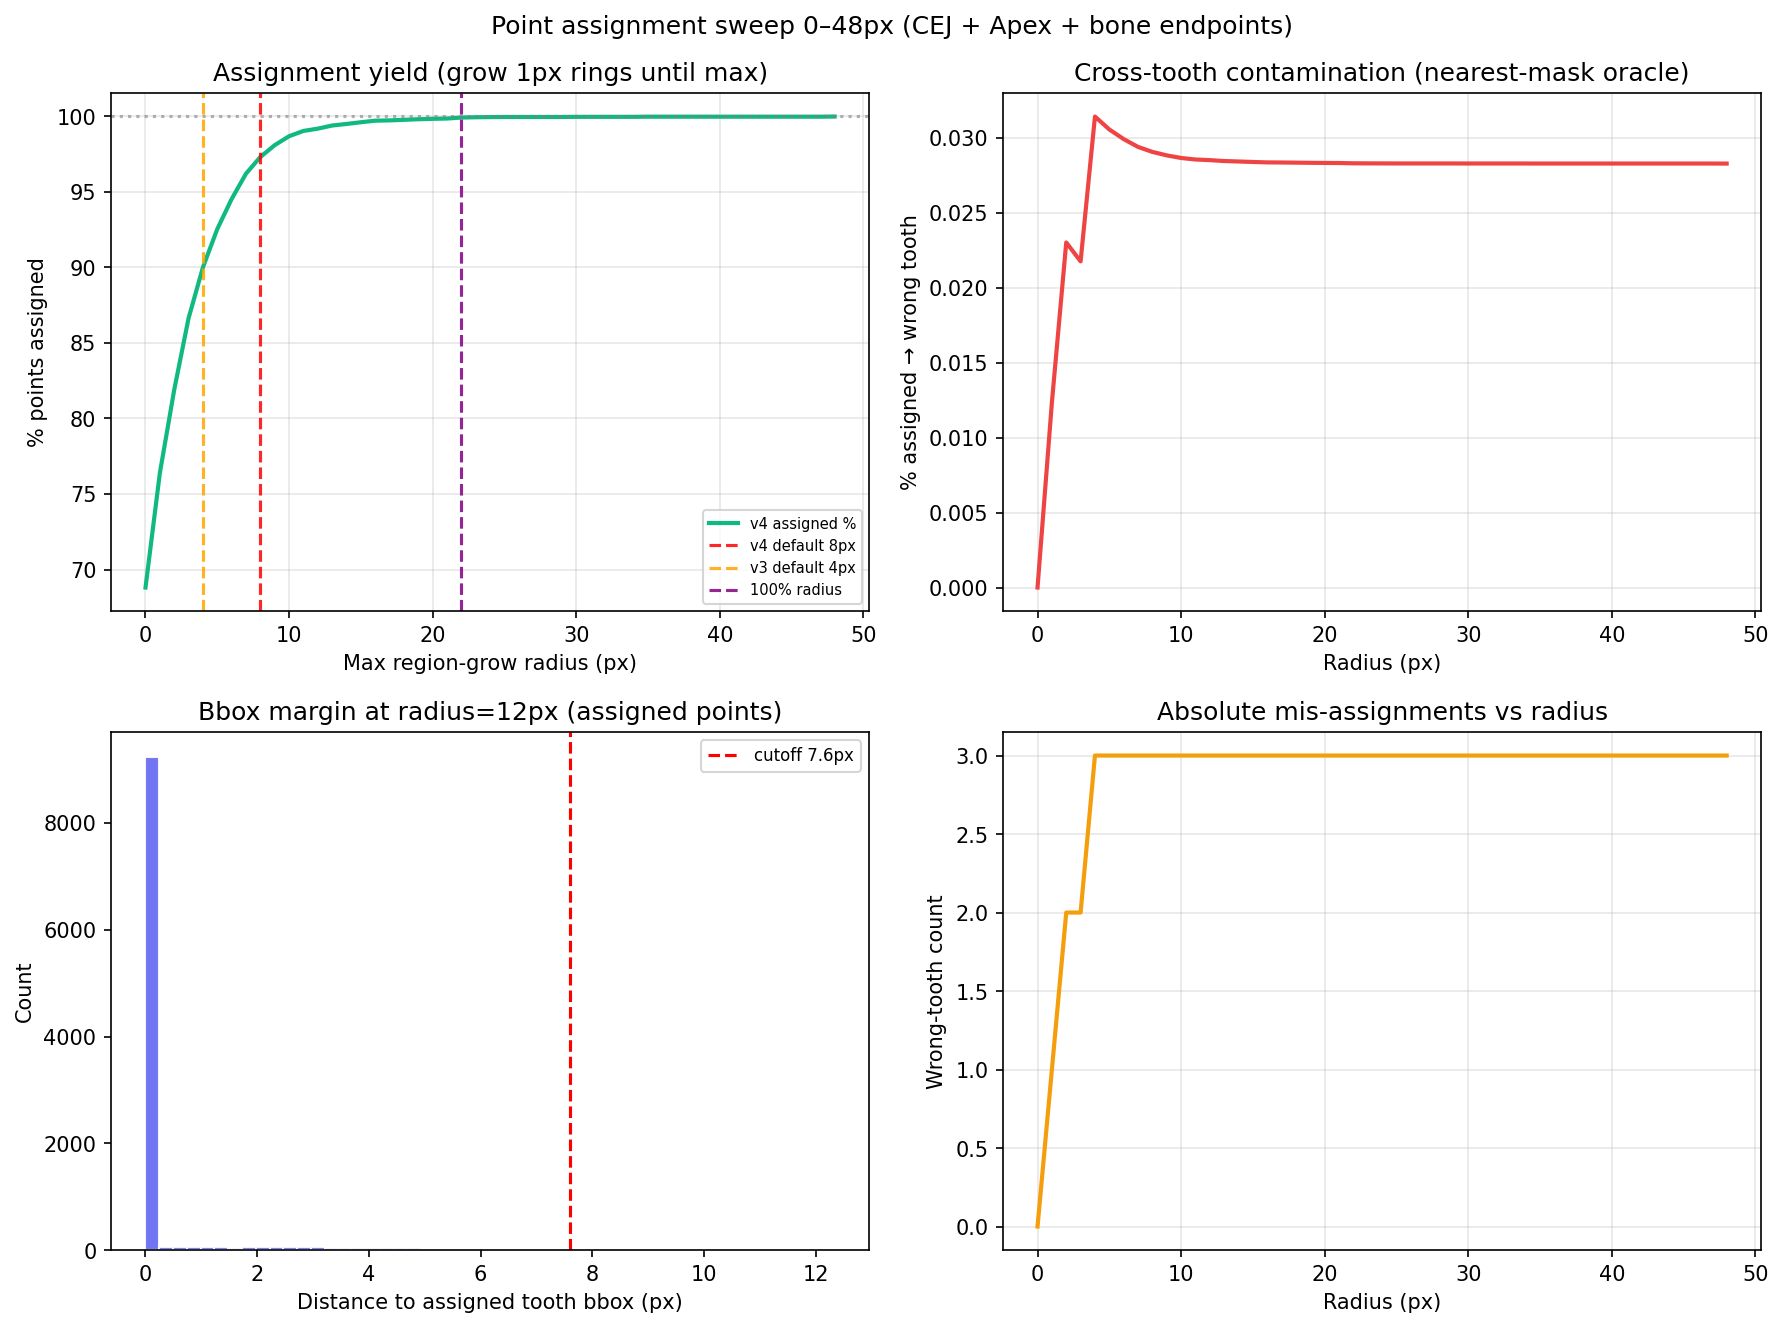
\includegraphics[width=\columnwidth]{point_assignment_full.png}
\caption{Assignment yield and cross-tooth contamination against the maximum ring radius, over all three splits. The pipeline uses 8\,px.}
\label{fig:grace}
\end{figure}

\subsection{Slot Assignment}

Each landmark class occupies two slots per tooth, mesial and distal. Assigning slots by horizontal image coordinate fails for tilted teeth. We assign them relative to the principal axis of the tooth mask, by the sign of the cross product between the axis direction and the vector from the mask centroid to the landmark. On identical ground-truth landmarks, severities computed under the two conventions are essentially uncorrelated (ICC $\approx -0.006$), so this is a different labelling scheme rather than a cosmetic change.

%==================================================================
\section{Severity Measurement}
\label{sec:method}

For a tooth side with CEJ $\mathbf{c}$, intersection $\mathbf{i}$ and apex $\mathbf{a}$, every definition below returns a percentage of root length. They differ only in how the measurement axis is constructed.

\subsection{Reference Definition}

The reference formula~\cite{denpar2026} sorts the three landmarks by horizontal coordinate, fits a line $\ell$ through them, and projects all three onto it:
\begin{equation}
S_{\text{ref}} = 100 \times \frac{\lVert \Pi_\ell(\mathbf{i}) - \Pi_\ell(\mathbf{c}) \rVert}{\lVert \Pi_\ell(\mathbf{a}) - \Pi_\ell(\mathbf{c}) \rVert},
\qquad \ell = \ell(\mathbf{c},\mathbf{i},\mathbf{a}).
\label{eq:ref}
\end{equation}
The apex enters twice: it helps determine $\ell$ and it sets the denominator. Writing $\varepsilon$ for a landmark perturbation,
\begin{equation}
\frac{\partial S}{\partial \varepsilon} =
\underbrace{\frac{\partial S}{\partial \mathbf{p}}}_{\text{displacement}} +
\underbrace{\frac{\partial S}{\partial \ell}\,\frac{\partial \ell}{\partial \varepsilon}}_{\text{rotation}}.
\label{eq:decomp}
\end{equation}
The first term is a bounded rescaling. The second is not: rotating $\ell$ moves the projections of landmarks that were themselves located correctly.

\subsection{Axis-Constrained Definition}

We fix the axis before the landmarks are read. Given an origin $\mathbf{o}$ and unit direction $\mathbf{u}$, each landmark reduces to a scalar coordinate $t(\mathbf{p}) = (\mathbf{p} - \mathbf{o}) \cdot \mathbf{u}$ and
\begin{equation}
S_{\text{axis}} = 100 \times \frac{\lvert t(\mathbf{i}) - t(\mathbf{c}) \rvert}{\lvert t(\mathbf{a}) - t(\mathbf{c}) \rvert}, \qquad S \in [0, 100].
\label{eq:axis}
\end{equation}
Two constructions of $(\mathbf{o},\mathbf{u})$ are evaluated. \textbf{Axis A} takes $\mathbf{o}$ as the mask centroid and $\mathbf{u}$ as the leading principal component of the mask pixel coordinates~\cite{jolliffe2002pca}; with $n \sim 10^4$ pixels the estimate is stable, and no landmark enters it, so $\partial\mathbf{u}/\partial\varepsilon = 0$ and the rotation term in~\eqref{eq:decomp} vanishes. \textbf{Axis B} takes $\mathbf{o}$ as the CEJ midpoint and $\mathbf{u}$ as the unit vector towards the intersection midpoint; it follows the clinical crest but depends on the predicted intersection landmarks. Fig.~\ref{fig:mechanism} shows both cases against the reference.

\begin{figure*}[t]
\centering

\includegraphics[width=0.92\textwidth]{T2_axis_mechanism.pdf}
\caption{Error propagation under the two axis constructions. Left: the reference line is refitted from the same perturbed landmarks it then projects, so noise both displaces the points and rotates the axis. Right: the mask principal axis is fixed by the segmentation, so only the scalar coordinates along a fixed direction move.}
\label{fig:mechanism}
\end{figure*}

A side is rejected as implausible when the intersection does not lie between the CEJ and the apex along the axis, with an 8\% slack of the root length at each end. The same rule is applied to~\eqref{eq:ref} so that all definitions are evaluated on comparable sides.

\subsection{What Is and Is Not Independent of the Apex}

The claim is specific. In Axis A and Axis B the apex contributes only to the denominator; the direction $\mathbf{u}$ is constructed without it. Apex error therefore rescales the value but cannot rotate the axis. This is an \emph{apex-independent axis}, not an apex-free measure: root length is defined by the apex, and a severity in raw pixels would not be comparable across teeth or magnifications. For completeness we also evaluate a genuinely apex-free \textbf{crown-width index}, which normalises the projected CEJ-to-intersection distance by the mesial--distal CEJ span. It is on a different scale and is never compared value-for-value with the root-length definitions.

%==================================================================
\section{Experimental Setup}
\label{sec:setup}

\textbf{Pipeline.} YOLOv8x detects teeth in two classes, single- and double-rooted, since the root class determines the number of apex slots. Detected regions are passed to three Keypoint R-CNN heads (ResNet-50 + FPN, two keypoints each), trained with Adam at $10^{-4}$, StepLR(4, 0.6), batch 2--4, CLAHE augmentation~\cite{lin2014clahe}, and early stopping on validation loss with patience 30. The heads are trained on ground-truth boxes and evaluated on detector boxes; this domain shift is a named contributor to the results in Section~\ref{sec:results}. Fig.~\ref{fig:arch} shows the full system.

\begin{figure*}[t]
\centering

\includegraphics[width=0.95\textwidth]{T1_system_architecture.pdf}
\caption{System architecture. The landmark heads are trained on ground-truth boxes but evaluated on detector boxes. The four severity definitions are computed from the same paired landmarks.}
\label{fig:arch}
\end{figure*}

\textbf{Metrics.} Detection uses precision, recall and mAP. Landmarks use a mean OKS per image with uniform falloff constants $\kappa_k = 1/K$, which is not COCO keypoint AP~\cite{anderson2019oks} and is the more forgiving of the two; reference values quoted from~\cite{denpar2026} are COCO AP and are shown only as an order-of-magnitude comparison. Severity agreement uses ICC(2,1), two-way random effects, absolute agreement, with percentile bootstrap 95\% confidence intervals over 2{,}000 resamples, mean absolute error, and Bland--Altman limits of agreement.

\textbf{Protocol.} Model and configuration selection use the validation split only; the test split is evaluated once per reported configuration. Predicted and reference tooth sides are paired by slot index, the strictest available protocol, since it penalises a mesial/distal swap.

\textbf{Hardware.} All training and evaluation ran on a single NVIDIA RTX 5070 (12\,GB). Its memory limit is the reason the keypoint batch size is below the reference's 8.

%==================================================================
\section{Results}
\label{sec:results}

\subsection{Label Construction}

Table~\ref{tab:labels} reports click retention and downstream landmark accuracy across label versions, with architecture and training schedule held fixed. The fixed 4\,px tolerance (v3) is a documented negative result: it improves CEJ retention and discards nearly a quarter of apex clicks. Region growing (v4) recovers both, and adding principal-axis slot assignment (v6) gives the production labels. From strict bounding-box assignment (v2) to v6 the gains are $+0.083$, $+0.080$ and $+0.083$ mean OKS for CEJ, intersection and apex.

\begin{table}[t]
\caption{Label construction: click retention and resulting landmark accuracy (mean OKS, test split).}
\label{tab:labels}
\centering
\resizebox{\columnwidth}{!}{%
\begin{tabular}{@{}l r r r r r@{}}
\toprule
\textbf{Version} & \textbf{CEJ loss} & \textbf{Apex loss} & \textbf{CEJ} & \textbf{INT} & \textbf{Apex} \\
\midrule
v2 strict box       & 5.6\% & 3.5\%  & 0.843 & 0.815 & 0.781 \\
v3 fixed 4\,px      & 1.9\% & \textbf{23.7\%} & 0.911 & 0.817 & 0.836 \\
v4 region growing   & \textbf{0.6\%} & \textbf{9.0\%} & 0.921 & 0.822 & 0.853 \\
v6 = v4 + PCA slots & 0.6\% & 9.0\%  & \textbf{0.926} & \textbf{0.895} & \textbf{0.864} \\
v7 12\,px + filter  & ---   & ---    & 0.928 & 0.882 & 0.881 \\
\midrule
Reference (COCO AP)~\cite{denpar2026} & & & 0.954 & 0.912 & 0.815 \\
\bottomrule
\end{tabular}}
\end{table}

Version v7 improves two of three classes and degrades the intersection. Severity is a conjunction of all three landmarks, and the intersection is its numerator, so selecting on the mean would optimise the wrong objective; v6 is used throughout.

\subsection{Detection}

The two-class detector reaches precision 0.850, recall 0.844, mAP@0.5 of 0.873 and mAP@0.5:0.95 of 0.794 on the test split, against the reference's 0.892, 0.963 and 0.907. The double-rooted class is the weaker (mAP@0.5 0.827 against 0.919), on 198 test instances against 666. A single-class variant reaches mAP@0.5 of 0.989 on validation; the task is strictly easier, since collapsing the classes removes the classification component of AP, and the figure is not comparable with the two-class results.

\subsection{Severity Agreement}

Table~\ref{tab:icc} is the central result. On identical landmarks and identical pairing, Axis A raises test ICC from 0.741 to 0.824. Its confidence interval lies almost entirely above that of the reference formula. All three definitions are near-unbiased; what separates them is spread, and the Bland--Altman limits narrow from 56 to 40 percentage points (Fig.~\ref{fig:ba}).

\begin{table}[t]
\caption{Severity agreement, test split. ICC(2,1) with bootstrap 95\% CI, MAE in percentage points, and Bland--Altman limits of agreement.}
\label{tab:icc}
\centering
\begin{tabular}{@{}l c c c r@{}}
\toprule
\textbf{Definition} & \textbf{ICC} & \textbf{95\% CI} & \textbf{MAE} & \textbf{LoA} \\
\midrule
Reference~\eqref{eq:ref} & 0.741 & [0.668, 0.807] & 7.22 & $[-28.6, 27.9]$ \\
\textbf{Axis A (mask)} & \textbf{0.824} & \textbf{[0.761, 0.880]} & \textbf{5.40} & $\mathbf{[-20.8, 18.9]}$ \\
Axis B (CEJ$\to$INT) & 0.770 & [0.702, 0.828] & 7.23 & $[-27.1, 27.0]$ \\
\midrule
Reference paper~\cite{denpar2026} & 0.801 & --- & --- & --- \\
\bottomrule
\end{tabular}
\end{table}

\begin{figure}[t]
\centering
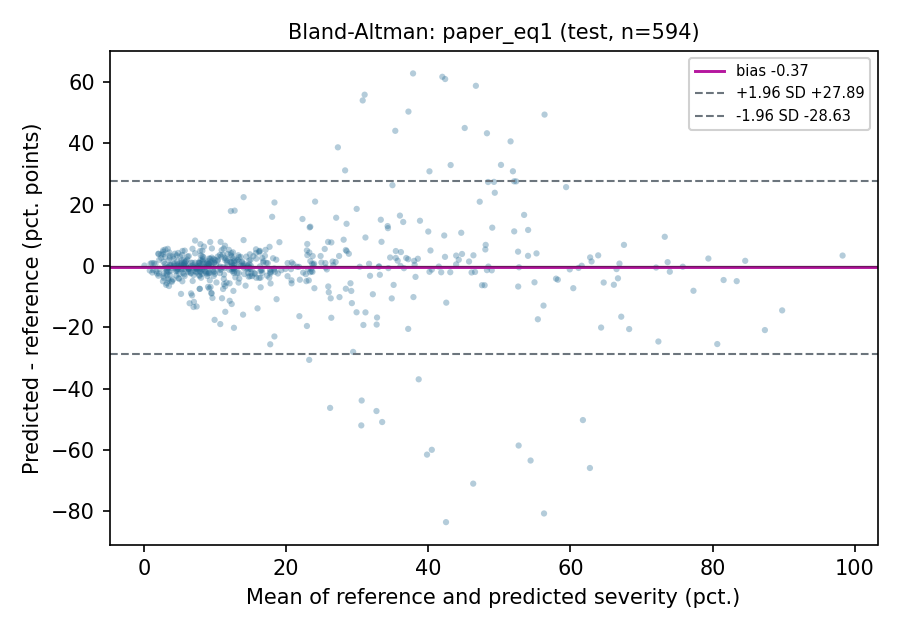
\includegraphics[width=0.49\columnwidth]{ba_ref.png}\hfill
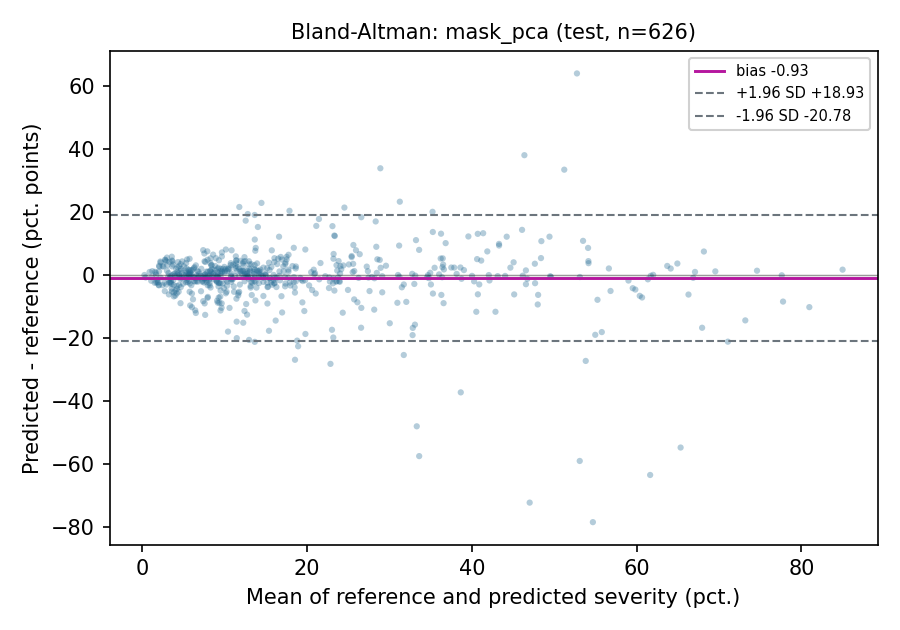
\includegraphics[width=0.49\columnwidth]{ba_pca.png}
\caption{Bland--Altman plots, test split. Reference formula (left) and Axis A (right). Both are near-unbiased; the limits of agreement are substantially narrower under the mask axis.}
\label{fig:ba}
\end{figure}

\textbf{Do the two formulas measure the same thing?} Computed on identical ground-truth landmarks with no model in the loop, the reference formula and Axis A agree at ICC 0.838 on test (MAE 2.46) and 0.931 on validation. The advantage in Table~\ref{tab:icc} therefore does not come from a different definition of bone loss. It appears only when the inputs are predicted, which is what~\eqref{eq:decomp} predicts.

\textbf{Is the advantage the rotation term?} Ground-truth landmarks were perturbed by isotropic Gaussian noise of known $\sigma$ and each definition re-measured against its own clean value, over ten realisations per $\sigma$ on the 200 test images, with teeth, masks and pairing held fixed (Table~\ref{tab:noise}, Fig.~\ref{fig:noise}). Axis A is the most robust definition at every non-zero noise level and its margin over the reference widens monotonically: $+0.014$ at 4\,px, $+0.018$ at 8\,px, $+0.041$ at 16\,px, $+0.051$ at 24\,px. A coincidence of one checkpoint would not produce a monotonic widening across a hundred independent realisations.

\begin{table}[t]
\caption{Robustness to injected landmark noise. ICC against each definition's own noise-free value; every column starts at 1.000.}
\label{tab:noise}
\centering
\begin{tabular}{@{}r c c c c@{}}
\toprule
$\sigma$ (px) & Reference & \textbf{Axis A} & Axis B & Crown-width \\
\midrule
2  & 0.989 & \textbf{0.999} & 0.990 & 0.999 \\
4  & 0.984 & \textbf{0.997} & 0.981 & 0.997 \\
8  & 0.972 & \textbf{0.989} & 0.963 & 0.988 \\
12 & 0.951 & \textbf{0.977} & 0.937 & 0.969 \\
16 & 0.921 & \textbf{0.962} & 0.894 & 0.947 \\
24 & 0.871 & \textbf{0.923} & 0.809 & 0.865 \\
\bottomrule
\end{tabular}
\end{table}

\begin{figure}[t]
\centering
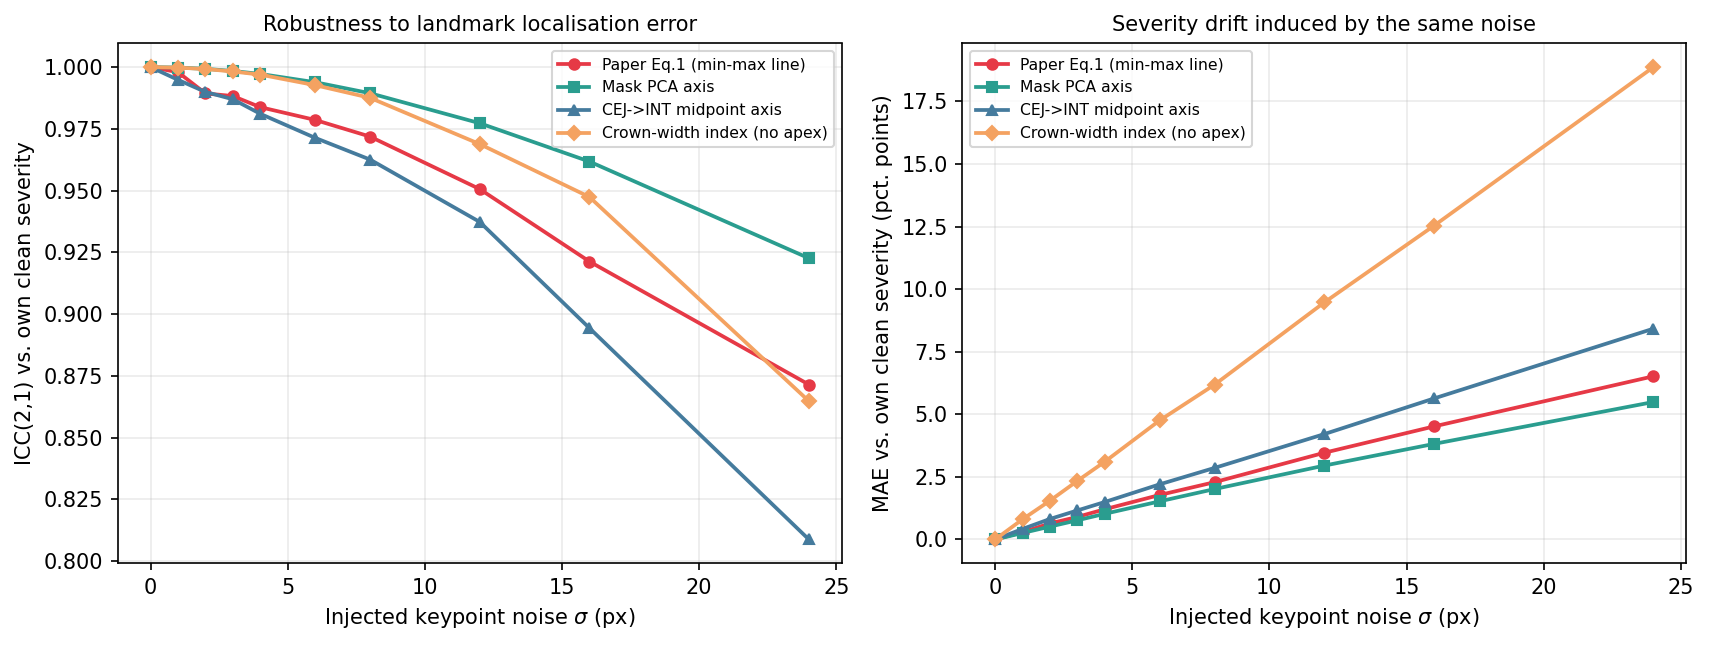
\includegraphics[width=\columnwidth]{noise_sensitivity.png}
\caption{Stability against injected landmark noise. Left: agreement with each definition's own clean value. Right: induced drift in percentage points; the crown-width index uses a smaller denominator, so its drift is not comparable across definitions.}
\label{fig:noise}
\end{figure}

The crown-width index, which uses no apex at all, exceeds the reference formula up to 16\,px and falls behind at 24\,px. Its numerator and denominator share the same CEJ landmarks, and that denominator is roughly half the root length, so removing the apex is not free: it trades an unreliable landmark for a smaller normaliser that shares its noise. Axis A is the better trade.

\textbf{Is the advantage specific to one model?} Re-running the pipeline with the v7 landmark heads, which localise the intersection less accurately (0.882 against 0.895), leaves the advantage intact: on test it grows from $+0.097$ to $+0.130$, as the mechanism predicts, since weaker landmarks supply more noise for a stable axis to absorb. Axis A is also the least sensitive definition to the substitution, losing 0.025 on test where the reference loses 0.058.

\textbf{Protocol sensitivity.} Across 126 configurations of landmark-combination strategy, side-pairing protocol and apex-merge radius, test ICC for the reference formula spans 0.559--0.727 (SD 0.062). The reference paper does not specify its pairing rule, so part of the gap to 0.801 is a protocol that had to be reinvented. The validation-selected configuration gives 0.7246 on test against a test-selected 0.7273; the lower number is reported.

\subsection{Coverage}

Severity requires all three landmarks on a side. Under the best label construction 27.7\% of teeth still carry no apex click, and severity is computable for 629 of 1{,}728 test tooth sides (36.4\%) under Axis A. This is an annotation ceiling, not a model failure, and it constrains the reference implementation identically. The system supports screening and within-patient comparison rather than comprehensive charting.

%==================================================================
\section{Discussion}
\label{sec:discussion}

Four factors account for the difference between the agreement reported here and the reference's 0.801: detection quality (0.873 against 0.963 mAP@0.5) together with the train-to-inference box domain shift; intersection localisation (0.895 against 0.912); the unspecified pairing protocol, worth SD 0.062; and annotation coverage. An oracle analysis with pairing assumed correct raises the reference formula to approximately 0.79, so the landmarks already carry most of the available information and the residual is dominated by matching. That finding redirected this work from improving the landmark models to improving the measurement geometry, where the gain proved larger.

Three limitations bound the claims. No clinical reader study was carried out; every reference severity is derived from dataset annotations, so the results establish agreement with an annotation protocol, not equivalence with clinical judgement, and limits of agreement of roughly $\pm 20$ percentage points remain wide for an individual treatment decision. All experiments use a single dataset from a single institution. And the reported OKS is a mean OKS with uniform falloff, not COCO AP, so the landmark comparison with the reference is not like-for-like.

%==================================================================
\section{Conclusion}
\label{sec:conclusion}

The reference formula for alveolar bone-loss severity lets the root apex determine the direction of measurement as well as its scale. Separating those roles, by deriving the axis from the tooth segmentation and keeping the apex only as the root-length denominator, raises test-split agreement with expert severity from ICC 0.741 to 0.824 on identical landmarks. The gain is a property of the geometry: the two formulas agree on identical ground truth, the advantage widens monotonically under injected noise, and it survives substitution of a weaker landmark model. Label construction, not architecture, limited landmark accuracy on this dataset, and annotation coverage, not model accuracy, limits how many teeth can be measured at all.

\bibliographystyle{IEEEtran}
\bibliography{references}

\end{document}
